\begin{figure}
\centering
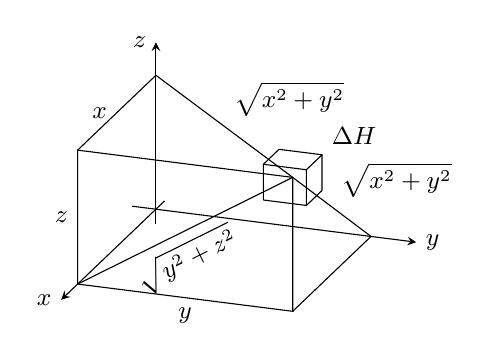
\begin{tikzpicture}[font=\small]
\pgfmathsetmacro{\a}{0.1}
\pgfmathsetmacro{\b}{0.2}
\pgfmathsetmacro{\c}{0.2}
\pgfmathsetmacro{\kx}{1}
\pgfmathsetmacro{\ky}{2}
\pgfmathsetmacro{\kz}{1.5}
\begin{axis}[clip=false,view/h=110,small,axis lines=center,xlabel={$x$},ylabel={$y$},zlabel={$z$},xlabel style={anchor=east},ylabel style={anchor=west},zlabel style={anchor=east},enlargelimits=true,xtick={\empty},ytick={\empty},ztick={\empty}]
\addplot3[]coordinates{(\kx-\a,\ky+\b,\kz-\c)(\kx-\a,\ky+\b,\kz+\c)(\kx-\a,\ky-\b,\kz+\c)};
\addplot3[]coordinates{(\kx+\a,\ky-\b,\kz-\c)(\kx+\a,\ky+\b,\kz-\c)(\kx+\a,\ky+\b,\kz+\c)(\kx+\a,\ky-\b,\kz+\c)(\kx+\a,\ky-\b,\kz-\c)};
\addplot3[]coordinates{(\kx-\a,\ky-\b,\kz+\c)(\kx+\a,\ky-\b,\kz+\c)};
\addplot3[]coordinates{(\kx-\a,\ky+\b,\kz+\c)(\kx+\a,\ky+\b,\kz+\c)};
\addplot3[]coordinates{(\kx-\a,\ky+\b,\kz-\c)(\kx+\a,\ky+\b,\kz-\c)};
\addplot3[]coordinates{(\kx,0,0)(\kx,\ky,0)(\kx,\ky,\kz)(\kx,0,\kz)(\kx,0,0)};
\addplot3[]coordinates{(\kx,\ky,0)(0,\ky,0)};
\addplot3[]coordinates{(\kx,0,\kz)(0,0,\kz)}node[pos=0.5,left]{$x$};
\addplot3[]coordinates{(0,0,\kz)(\kx,\ky,\kz)}node[pos=0.5,above right]{$\sqrt{x^2+y^2}$};
\addplot3[]coordinates{(\kx,\ky,\kz)(0,\ky,0)}node[pos=0.5,above right]{$\sqrt{x^2+y^2}$};
\addplot3[]coordinates{(\kx,\ky,\kz)(\kx,0,0)}node[pos=0.55,sloped,below]{$\sqrt{y^2+z^2}$};
\RightAngle{(\kx,\ky,\kz)}{(\kx,0,\kz)}{(0,0,\kz)}
\addplot3[draw=none]coordinates{(\kx,0,0)(\kx,0,\kz)}node[pos=0.5,left]{$z$};
\addplot3[draw=none]coordinates{(\kx,0,0)(\kx,\ky,0)}node[pos=0.5,below]{$y$};
\addplot3[]coordinates{(\kx-\a,\ky+\b,\kz+\c)}node[above right]{$\Delta H$};
\end{axis}
\end{tikzpicture}
\end{figure}

\begin{figure}
\centering
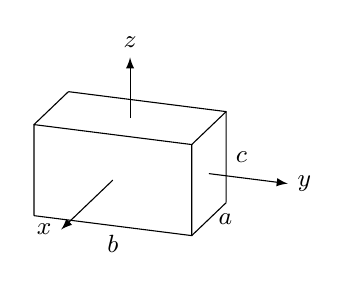
\begin{tikzpicture}[font=\small]
\pgfmathsetmacro{\a}{1}
\pgfmathsetmacro{\b}{2}
\pgfmathsetmacro{\c}{1.5}
\pgfmathsetmacro{\kx}{0}
\pgfmathsetmacro{\ky}{0}
\pgfmathsetmacro{\kz}{0}
\begin{axis}[clip=false,view/h=110,small,axis lines=center,xlabel={$x$},ylabel={$y$},zlabel={$z$},xlabel style={anchor=north},ylabel style={anchor=west},zlabel style={anchor=east},enlargelimits=true,xtick={\empty},ytick={\empty},ztick={\empty},hide axis]
\addplot3[]coordinates{(\kx-\a,\ky+\b,\kz-\c)(\kx-\a,\ky+\b,\kz+\c)(\kx-\a,\ky-\b,\kz+\c)};
\addplot3[]coordinates{(\kx+\a,\ky-\b,\kz-\c)(\kx+\a,\ky+\b,\kz-\c)(\kx+\a,\ky+\b,\kz+\c)(\kx+\a,\ky-\b,\kz+\c)(\kx+\a,\ky-\b,\kz-\c)};
\addplot3[]coordinates{(\kx-\a,\ky-\b,\kz+\c)(\kx+\a,\ky-\b,\kz+\c)};
\addplot3[]coordinates{(\kx-\a,\ky+\b,\kz+\c)(\kx+\a,\ky+\b,\kz+\c)};
\addplot3[]coordinates{(\kx-\a,\ky+\b,\kz-\c)(\kx+\a,\ky+\b,\kz-\c)};
\addplot3[-latex]coordinates{(\a,0,0)(\a+3,0,0)}node[left]{$x$};
\addplot3[-latex]coordinates{(0,\b,0)(0,\b+2,0)}node[right]{$y$};
\addplot3[-latex]coordinates{(0,0,\c)(0,0,\c+2)}node[above]{$z$};
\addplot3[]coordinates{(\a,0,-\c)}node[below]{$b$};
\addplot3[]coordinates{(0,\b,-\c)}node[right]{$a$};
\addplot3[]coordinates{(-\a,\b,0)}node[right]{$c$};
\end{axis}
\end{tikzpicture}
\end{figure}



\begin{figure}
\centering
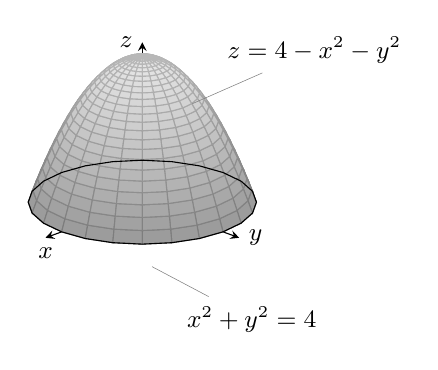
\begin{tikzpicture}[font=\small,declare function={fx(\r,\t)=\r*cos(\t);fy(\r,\t)=\r*sin(\t);fz(\t,\t)=4-(\r)^2;}]
\pgfmathsetmacro{\ra}{1.2}
\pgfmathsetmacro{\ta}{45}
\begin{axis}[clip=false,view/h=135,small,axis lines=center,xlabel={$x$},ylabel={$y$},zlabel={$z$},xlabel style={anchor=north},ylabel style={anchor=west},zlabel style={anchor=east},enlargelimits=true,xtick={\empty},ytick={\empty},ztick={\empty},colormap={}{gray(0cm)=(0.6);gray(1cm)=(0.9);}]
\addplot3[z buffer=sort,surf,domain=0:2,domain y=0:360,variable=\r,variable y=\t]({fx(r,t)},{fy(r,t)},{fz(r,t)});
\addplot3[domain y=0:360,variable=\r,variable y=\t]({fx(2,t)},{fy(2,t)},0);
\addplot3[]coordinates{(0,1,3)}node[pin=45:{$z=4-x^2-y^2$}]{};
\addplot3[]coordinates{(2,2,0)}node[pin=-45:{$x^2+y^2=4$}]{};
\end{axis}
\end{tikzpicture}
\end{figure}
